\documentclass[11pt,en]{elegantpaper}

\makeatletter

\renewcommand\paragraph{\@startsection{paragraph}{4}{\z@}%
            {-2.5ex\@plus -1ex \@minus -.25ex}%
            {1.25ex \@plus .25ex}%
            {\normalfont\normalsize\bfseries}}
\makeatother
\setcounter{secnumdepth}{4} % how many sectioning levels to assign numbers to
\setcounter{tocdepth}{4}    % how many sectioning levels to show in ToC
\title{High School Math Learning Resource Recommendation Based on Knowledge Tracing and Factorization Machines}
\author{Wangzhihui Mei}
\institute{CCNU-JI}

\date{}

% cmd for this doc
\usepackage{array}
\newcommand{\ccr}[1]{\makecell{{\color{#1}\rule{1cm}{1cm}}}}

\begin{document}

\maketitle

\begin{abstract}
	This paper implements a high school mathematics learning resource recommendation system based on knowledge tracking and factorization machine, which contains three core points. The first one is the design of data source, and proposes an automatic extraction method for test knowledge points. The whole process of high school mathematics knowledge mapping from corpus collection, construction, storage, and update is introduced as well as the automation process. The second point is the implementation of a GCN-based knowledge tracking algorithm, which takes into account the a priori structure of knowledge points as well as students' recent question records and knowledge mastery changes, and achieves a more excellent performance compared to other knowledge tracking models. The third point is based on a deep factorization machine, which solves the problem of sparsity of training data, and it takes the output of the knowledge tracking model as input and considers various other feature inputs to achieve learning resource recommendation.
\keywords{Learning Resource Recommendation System, Knowledge Graph, Knowledge Tracing, Factorization Machine}
\end{abstract}


\section{Introduction}
\subsection{Research Background and Significance}
Artificial intelligence industry has developed rapidly in recent years, it is being commercialized in all aspects, triggering profound changes in various industries, and the future development of artificial intelligence will be the combination of key technologies and industries.\cite{cui2018performance} At present, AI technology has been implemented in many fields such as finance, medical and security, and the application scenarios are becoming more and more abundant. The commercialization of AI has played a positive role in accelerating the digitization of enterprises, improving the structure of the industrial chain, and increasing the efficiency of information utilization. The traditional education industry also tries to use AI technology to help the development of the industry. Every development of AI is accompanied by breakthroughs in research methods, and deep learning is one of the important representatives of the breakthroughs in machine learning technology in recent years. With the continuous extension of human AI research and application fields, AI will usher in more kinds of technology combination applications in the future. Artificial intelligence has also begun to be applied to the education industry, and the concept of intelligent education has emerged. Among the types of applications of AI technology in education, AI adaptive learning is the most widely used in all aspects of learning. In addition, due to China's large population base, the shortage of educational resources, the importance attached to education and other favorable factors intelligent adaptive learning system is expected to come later. 

In recent years, domestic adaptive learning has begun to enter the minds of many people involved in education training and education investment. There are more and more education technology companies in the market that focus on adaptive learning tools. At the same time, many education companies have started to use adaptive learning as the main core function or main selling point of their products. The biggest advantage of adaptive education is that it can locate the knowledge gaps of each student. The adaptive learning platform will guide the student to the next most suitable learning content and activities for him. When students encounter a course that is too difficult or too low in the learning process, they can automatically adjust the difficulty of the course. Teachers can also analyze the knowledge gaps of each student based on the learning status evaluation report provided by the system, adjust the learning progress in real time, and provide personalized teaching for each student. So theoretically, adaptive learning is one of the potentially feasible solutions to the problem of "teaching to students according to their abilities" in online education. To make a practical adaptive learning system, I plan to use knowledge tracing to track students' learning status and use the factorization machine algorithm to calculate the relevance of topics to students to build such a test recommendation system.The current personalized learning resource recommendation system is one way of implementing adaptive learning, which is the subject of this paper.

In this paper, the study focuses on the recommendation of learning resources for the subject of high school mathematics. In this system, there are two aspects in general: on the one hand, scientific and targeted acquisition and tracing of students' knowledge state, and on the other hand, recommendation of personalized learning resources based on students' knowledge mastery state. We use the knowledge tracing algorithm of graph neural network to acquire and track students' knowledge states, and the factorization agent to try to combine the output of graph neural network with prior knowledge for resource recommendation.


\subsection{Research Status}
The dominant content of the research is knowledge tracing and recommendation system. Some advanced graph neural network algorithm is applied to finish the task. There have been some research advances and related applications in the area of knowledge tracing and factorization. We surveyed some existing knowledge tracing algorithms and applications, and some applications of factorization machine.

\subsubsection{Property of high school Math}
Disciplines and knowledge are closely related to each other, so that disciplinary knowledge denotes the specific knowledge contained in a particular field of study. Disciplines are referred to in this study only for specific subjects in the field of education, such as mathematics, language, chemistry and so on. The first step is to learn how to make the best use of the knowledge that is available. The knowledge is obtained from practice, so after learning it, it can also be applied to social practice. Scientific knowledge is declarative because it can be expressed in a series of symbols, words and diagrams; it is also procedural because it can be arranged and learned according to a specific logical order in the process of concrete learning.

Mathematics is a science specializing in the study of the relationship between quantities and spatial forms, its symbolic system is more complete, the formula structure is clear and unique, text and images and other expressions of language is also more vivid and intuitive.

The knowledge that learners need to learn mostly comes from the summaries of the experiences of their predecessors in practical activities. The learning process is a process of cognitive learning of the summarized knowledge and continuous digestion, adjustment and reorganization of the knowledge structure, so as to build a more perfect and suitable knowledge structure, as well as a process of integration with innovative thinking. Thus a good cognitive structure can promote the formation of knowledge structure, and a good knowledge structure can enrich the organization form of cognitive structure. Since the disciplinary knowledge structure consists of two parts: knowledge composition and knowledge dependency, we will analyze the disciplinary knowledge structure from these two aspects, knowledge structure and composition.

The knowledge that learners need to learn mostly comes from the summaries of the experiences of their predecessors in practical activities. The learning process is a process of cognitive learning of the summarized knowledge and continuous digestion, adjustment and reorganization of the knowledge structure, so as to build a more perfect and suitable knowledge structure, as well as a process of integration with innovative thinking. So a good cognitive structure can promote the formation of knowledge structure, and a good knowledge structure can enrich the organization form of cognitive structure. Since the disciplinary knowledge structure consists of two parts: knowledge composition and knowledge dependency, we will analyze the disciplinary knowledge structure from these two aspects.

Knowledge composition refers to the organization of knowledge within a subject area, which mainly includes knowledge points, knowledge blocks and knowledge systems. 
\begin{itemize}
	\item knowledge point: A point of knowledge is the smallest constituent unit of the knowledge structure of a discipline and is used to represent specific concepts. 
	\item knowledge block: A knowledge block is a collection of one or more sets of knowledge points, also known as knowledge modules, in which knowledge blocks and knowledge blocks can be combined to form new knowledge modules, and a subset of knowledge blocks is called a knowledge sub-module.
	\item knowledge body: a body of knowledge is a structured system that is a combination of all the pieces of knowledge in a particular subject area.
\end{itemize}


Mathematics is a science that specializes in the relationship between quantity and spatial form. Its symbol system is more complete, the formula structure is clear and unique, and the language of expression such as words and images is more vivid and intuitive. The knowledge structure of senior secondary mathematics is a more logical and systematic knowledge system organized on the basis of the knowledge structure of junior secondary mathematics. This is because learning for any discipline needs to be based on the existing cognitive structure in order to progressively effective learning and skills training, so in the process of learning high school mathematics, you need to have a solid foundation of junior high school mathematics discipline knowledge. In the past few years, there have been a number of cases in which the students have been able to learn from each other.

\begin{itemize}
	\item Highly abstract: Mathematics has a high degree of abstraction, because the discipline's knowledge system is built using many abstract knowledge concepts, and with the help of these concepts and knowledge to learn and expand thinking, forming new abstract conceptual knowledge. The abstraction of mathematics is reflected in the object is not concerned with the introduction of specific content, only the number of relationships between the spatial form. Therefore, abstraction in mathematics is different from abstraction in other disciplines in terms of both object and degree. There are also some differences between mathematics and the natural sciences, because in mathematics the accuracy of calculations, proofs, and inferences can only be verified using rigorous logical methods and cannot be tested by repetitive experiments, whereas in the natural sciences the verification is the opposite.
	\item Strict logic: The discipline of mathematics is very logical because any conclusion reached in mathematics requires rigorous logical reasoning and rigorous proof in order to be considered reasonable. However, mathematics is not the only discipline that possesses rigorous logic; other natural science studies of reasoning and proof must also possess a certain degree of logic. In mathematics, not all conclusions reached after reasoning and proof can be applied in practice, because many mathematical models are developed and mathematical conclusions drawn under ideal circumstances.
	\item Broad applicability: Mathematics is an important means and tool for us to participate in practical social activities or scientific research, and the study of mathematics is indispensable in all walks of life and in all areas of society. Therefore, mathematics has a wide range of applications and has become an important basis for the development of modern science.
\end{itemize}

\subsubsection{Knowledge relation}
Knowledge relations represent the connections between knowledge points (or between knowledge blocks and knowledge chunks) in the discipline knowledge structure. It is through these connections that different knowledge points can be formed into knowledge blocks, and different knowledge blocks can be combined to form the whole disciplinary network knowledge structure system. There are many different kinds of knowledge relationships, so that different definitions of knowledge relationships lead to different knowledge structures. Therefore, in order to unify the definition of knowledge relations, we divided them into general relations and special relations based on the general and special characteristics of discipline knowledge structure. The special relationships represent the unique knowledge relationships of a particular discipline, while the universal relationships represent the general relationships of any discipline. Secondly, according to the demands of knowledge graphping research, we divide universal relations into six kinds of knowledge relations: synonymous, fraternal, antecedent, consequent, inclusive and antagonistic; and special relations into four kinds of knowledge relations: detailed, transformative, causal and correlative.
\begin{itemize}
	\item tautology: Expresses the relationship between two points of knowledge that have the same meaning as what is being described, e.g. regular and equilateral triangles.
	\item fraternity: Expresses the relationship between two knowledge points that have the same parent class.
	\item predecessor: It means that you need to finish learning knowledge point A before learning knowledge point B, that is, $A\rightarrow B$ is a precursor relationship.
	\item successor: denotes the inverse of the antecedent relationship, i.e., $B\rightarrow A$ is the successor relationship.
	\item containment: Indicates that knowledge point B is included in the definition of knowledge point A, i.e., $A\rightarrow B$ is an inclusion relationship.
	\item antagonism: From a certain point of view, knowledge point A is incompatible with knowledge point B, i.e. $A\leftrightarrow B$ is an antagonistic relationship.
	\item refinement: A grammatical analysis of the definition of knowledge point A leads to knowledge point B, where $A\leftrightarrow B$ is a detailed relationship
	\item transformation: denotes that knowledge point A and knowledge point B can be transformed to each other under certain conditions, i.e., $A\leftrightarrow B$ is a transformation relationship.
	\item causation: denotes that knowledge point A can be deduced from knowledge point B as a known condition, i.e., $A\leftrightarrow B$ is a causal relationship. 
	\item relation: Indicates that there is a relationship between the definitions of Knowledge Point A and Knowledge Point B, but the relationship is not explicitly specified, i.e., $A\leftrightarrow B$ are correlated.
\end{itemize}

In the process of constructing the discipline knowledge structure, firstly, we need to analyze the current discipline knowledge content, teaching objectives, teaching objects, teaching strategies and discipline characteristics in detail; secondly, we divide the whole discipline knowledge system into several knowledge modules, and then we divide each knowledge module into several knowledge points; finally, with reference to the above ten kinds of knowledge relationships and the knowledge relationships extracted from data sources, we can determine and establish the relationships between knowledge modules and knowledge modules, between knowledge modules and knowledge points, and between knowledge points and knowledge points, so as to form a complete discipline knowledge system structure.



\subsubsection{Knowledge tracing algorithms}
Knowledge Tracing is a technique that models students' knowledge acquisition based on their past answers to obtain a representation of their current knowledge state. The task is to automatically track the change of students' knowledge level over time based on their historical learning trajectory, in order to be able to accurately predict the students' performance in future learning and to provide appropriate learning tutoring. In this process, the knowledge space is used to describe the level of student knowledge acquisition. A knowledge space is a collection of concepts, and a student's mastery of a part of a collection of concepts constitutes the student's mastery of knowledge. Some educational researchers argue that students' mastery of a particular set of related knowledge points will affect their performance on the exercise, i.e., the set of knowledge that students have mastered is closely related to their external performance on the exercise.

The task of knowledge tracing is to model the student's knowledge mastery state based on the student's answer record, which is usually a time series, and in some business scenarios is time-independent, so that we can accurately predict their future answers and make reference for future intelligent questioning based on this to avoid giving students too difficult or too easy questions. Specifically, suppose a student's answer record is $x_0,x_1,...,x_t$, and we are going to predict the next interaction $x_{t+1}$, usually one interaction $x_t=(q_t,a_t)$, $q_t$ represents the right or wrong situation of that student's answer to the question $a_t$.

There are several kinds of knowledge tracing algorithms: 
\begin{itemize}
	\item Bayesian knowledge tracing(BKT): Bayesian knowledge tracing is an early and commonly used knowledge tracing model, BKT uses user interaction modeling with real-time feedback to model a learner's potential knowledge state as a set of binary variables, each representing whether or not a knowledge point is understood, and there are dynamic changes in mastery of knowledge points as students continue to practice, BKT maintains binary variables of knowledge point proficiency by using Hidden Markov Models (HMM), the original BKT model does not take into account students' knowledge forgetting, and related studies address students' guesses, personal vivid knowledge mastery and problem difficulty factors on BKT\cite{yudelson2013individualized}. 
	\item Deep Knowledge Tracing(DKT): The DKT model applies neural networks to the knowledge tracing task for the first time\cite{piech2015deep}, using an LSTM model to track the dynamics of student knowledge proficiency over time, and to learn the potential vector representation of student knowledge proficiency directly from the data. The advantage of DKT is that it can record knowledge over a longer period of time based on students' recent answers. In addition, it can update the knowledge state based on each answer, only the last implicit state needs to be saved, no double counting is required, and it is suitable for online deployment. It does not require domain knowledge, works with any user answer dataset and automatically captures associations between similar questions. The disadvantage of DKT is that the model output fluctuates greatly when the answer sequence is disrupted, i.e., the same questions and the same responses yield different knowledge states when the answer sequence is inconsistent. Due to the above-mentioned problems and the fact that students do not necessarily have continuous consistency in their k
	nowledge during the answer process, it leads to bias in the prediction of students' knowledge states influenced by the sequence. There is also the black box problem, which sometimes leads to the strange situation that the first correct answer leads to a high prediction probability for all subsequent ones, while the first wrong answer leads to a low prediction probability for all subsequent ones.
	\item Dynamic Key-Value Memory Networks for Knowledge Tracing(DKVMN): Dynamic Key-Value Memory Networks for Knowledge Tracing (DKVMN) was proposed in 2017 by Jian Jian of the Chinese University of Hong Kong\cite{zhang2017dynamic}. Based on the strengths and weaknesses of BKT and DKT and using the memory augmentation neural network approach, the Dynamic Key-Value Memory Networks (DKVMN) is proposed. It borrows ideas from memory-enhanced neural networks and combines the advantages of BKT and DKT. DKVMN stores all knowledge points with a static matrix key and a dynamic matrix value to store and update the student's knowledge state. In the DKVMN paper, they compare DKVMN with DKT and a sophisticated version of BKT, BKT+. They found that DKVMN achieves excellent performance and is the most advanced model in the KT domain. In addition to improved performance, it has several other advantages over LSTM, including prevention of overfitting, a smaller number of parameters, and automatic discovery of similar practice questions by underlying concepts. In addition, Chaudhry R\cite{chaudhry2018modeling} improves the performance of DKVMN by jointly training request cue prediction with knowledge tracing through multi-task learning.
\end{itemize}

\subsubsection{Factorization Machine}
The factorization machine model is a factorization model that can be used in large scale sparse data scenarios\cite{rendle2010factorization}. The solution of this model is linear in time complexity and he can solve it directly using raw data without relying on support vectors like SVM. In addition, FM is a general model that can be used on any real data and can do tasks such as classification and regression and even sorting. The idea is that the idea is to add a linear combination of two features to linear regression, and the way to solve the linear combination is to use a matrix decomposition. FFM is an improvement on FM by adding the concept of Field\cite{juan2016field}, that is, the class to which each feature belongs. Suppose there are f Fields. Then each feature has to have f hidden vectors. When two features are crossed, the dot product of each feature and the vector corresponding to the other Field is used. In this way, it is ensured that the same Field does the same thing for the same feature, and the features of different Fields do different things for the same feature. In addition, there is also a deep learning version of the factorization machine algorithm\cite{guo2017deepfm}, and this model is improved based on wide and deep. First, the model includes FM and DNN parts, which is a parallel structure, and FM and DNN share the same input (embedding). The mapping vector from the field to the embedding layer is exactly the vector learned by the FM layer. It has the advantage that it does not require pre-training and can learn the intersection of low and high dimensional features.
\subsection{Research Content}
The purpose of this study is to build a high school mathematics learning resource recommendation system based on knowledge tracing and factorization machine algorithm. We use knowledge tracing to model students' knowledge states, which outputs a graphical knowledge state vector, which we use as the next-level input, considering students' individualized differences and knowledge forgetting process, and apply the factorization machine algorithm to the resource recommendation system. For knowledge tracing, we build a graph neural network-based knowledge tracing model, which can well characterize the intrinsic connections of knowledge points in mathematics subjects considering that the knowledge points are a graph-like structure, and output a graph knowledge vector matrix, which can also effectively characterize the connections between problems and knowledge points. The output of the knowledge tracing model is then passed through a factorization machine algorithm to obtain the recommendation degree of the learning resources and output a vector of recommendation weights for different learning resources.

\subsection{Structure}
Chapter 1 of this paper is an introduction. It introduces the research background of the study, current industry-related research progress and the focus of the study. Then it leads to the three core points of this paper: learning resource representation, knowledge tracing and resource recommendation.

Chapter 2 of this paper concentrates on learning resource representation, which addresses storing learning resources through knowledge graphs. This paper explores some concepts of knowledge graphs, related studies, and then gives the process of knowledge graph building. It is also demonstrated that knowledge graph building can effectively characterize the a priori intrinsic features of subject knowledge.

Chapter 3 of this paper gives a knowledge tracing model of pre-trained graph neural network, which better characterizes the graph-like properties of knowledge. It is able to transform the knowledge tracing task into a time-series node-level classification problem in GNNs. Since the knowledge graph structure is not explicitly provided in most cases, we present various implementations of the graph structure. Empirical tests on two open datasets show that the method improves the prediction of student performance without any additional information and shows more interpretable predictions. The inclusion of pre-training is also attempted during the experiments, which can greatly improve the training efficiency and performance.

Chapter 4 of this paper proposes the application of a deep factorization machine algorithm with knowledge tracing model data as input to build a learning resource recommendation system. The output is a weight vector of top n, characterizing the recommended resources of top n.

Chapter 5 of this paper presents the conclusion.

\clearpage
\section{The Knowledge Graph of High School Math}
\subsection{Motivation and Contribution}
In this section, this paper uses the knowledge graph to store the knowledge points and questions of high school mathematics as the data source for the recommendation system. It serves as a supplementary input to the knowledge tracing model section and provides a priori knowledge of the subject knowledge points.

Firstly, the basic principles and common techniques of knowledge graph are introduced, and then a knowledge graph construction method for automatic extraction of knowledge points of test questions is proposed, and the knowledge graph construction and knowledge point extraction, corpus acquisition and preprocessing, knowledge point identification and knowledge graph updating techniques are introduced.

In the paper "Design and Implementation of Full Knowledge Graph for Middle School Mathematics Problems", Zhu Youjuan analyzed and studied the strategy of using ontology to build knowledge graphs. In the paper, Zhong Liang et al. used junior high school mathematics textbooks as the reference basis to collect data on relevant topics from Baidu Encyclopedia by writing a web crawler program, and downloaded knowledge data of high school mathematics subjects by accessing the Chinese Wikipedia download library. The data corpus was processed by writing relevant algorithms and programs to extract and correct the concepts and concept relationships related to the subject area of middle school mathematics. Finally, all the data are analyzed and integrated, and the data are used to construct a knowledge graph of junior high school mathematics.

In this paper, we will use the knowledge graph in constructing the knowledge graph of mathematics domain and building the student user model. In the construction of the knowledge graph of high school mathematics domain, the basic concepts and keywords involved in the textbooks are abstracted into knowledge point ontologies, the knowledge point keywords in high school mathematics exercises are identified by the named entity recognition method, and then the abstracted knowledge points are associated with the keywords to build the knowledge graph of high school mathematics. A large number of knowledge points in high school mathematics are associated with the degree of mastery of each knowledge point by individual students, which is built into a student user model, and the abstraction of the student user model into a knowledge graph will facilitate the personalized recommendation of exercises.

\subsection{Basic theory of knowledge graph}
The Knowledge Graph is a new concept introduced by Google in 2012. Knowledge graph is essentially a knowledge base of Semantic Network, which describes conceptual entities and their relationships in the objective world in a structured form. From the beginning of oogle search, to nowadays chatbots, big data risk control, securities investment, intelligent medical care, adaptive education, recommendation system, all use knowledge graph.
\subsubsection{Knowledge graph representation}
Knowledge graphs focus on concepts, entities and their relationships, where entities are things in the objective world and concepts are generalizations and abstractions of things with the same properties. Ontology is the basis of knowledge representation of knowledge graph, which can be formally represented as $O=\{C,H,P,A,I\}$, where $C$ is the set of concepts, such as transactional concepts and event-like concepts, $H$ is the set of contextual relations of concepts, $P$ is the set of attributes, which describes the features possessed by concepts, $A$ is the set of rules, which describes the domain rules, and $I$ is the set of instances, which describes the instance-attribute-value.

The common knowledge graph representations are Resource Description Framework (RDF), Resource Description Framework Schema (RDFS), Web Ontology Language (OWL), etc.

\begin{enumerate}
\item resource description framework RDF is the most commonly used symbolic semantic representation model, which provides a unified standard for describing entities/resources. the basic model of RDF is a directed labeled graph, each edge on the way corresponds to a subject-predicate object triad, and a triad corresponds to a statement of an event. the RDF consists of nodes and edges, the nodes represent entities/resources, attributes, and the edges represent entities and the relationship between entities and attributes. Figure \ref{triad1} shows the relationship between entities and attributes.
\item lightweight schema language RDFS is an extension of RDF by adding the definition of class properties and other Schema layers on top of the objective events provided by RDF. rdfs is mainly used to define term sets, class sets and property sets, mainly including classes, subclasses, properties, subclass properties, domains, scopes and other primitives, which can build the basic class hierarchy and These clauses can build the basic class hierarchy and attribute system.
\item OWL is the core of the Semantic Web technology stack, which provides fast and flexible data modeling capability and efficient automatic reasoning capability.
\end{enumerate}

\begin{figure}[h]
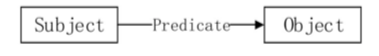
\includegraphics[width=0.8\textwidth]{./image/f01.png}
\caption{Structure of Triad}
\label{triad1}
\end{figure}

\subsubsection{Knowledge graph storage}
There are mainly two kinds of storage for knowledge graphs, one is based on the academic idea of RDF, which is based on triples car storage: the other is based on the industrial idea of attribute graph, which is based on attribute graph storage.

Using RDF for storage, mainly RDF serialization methods, such as RDF/XML, N- Triples, Turtle, RDFa, JSON-LD, etc.

The most important feature of the graph database for storing knowledge graphs is that the graph database can store not only the nodes and relations of triples, but also the attributes of their nodes and relations together, and the graph can be traversed efficiently, which is convenient for publishing data and retrieval of knowledge graphs.

\subsection{Constructing the Knowledge Graph}
In order to convert a large number of standard questions into feature questions in a timely manner, this paper proposes an automatic knowledge extraction method based on knowledge graph for test questions. The method uses natural language processing techniques such as named entity recognition, keyword extraction and calculation of semantic similarity of keywords to collect knowledge points and mathematics-related vocabulary in high school mathematics domain and build up a knowledge map of high school mathematics. The mathematics test questions are divided into words and entities by customized dictionaries and rules, and the candidate keywords are extracted and brought into the knowledge map of high school mathematics for querying.

\subsubsection{The extraction of knowledge point}
In this paper, the architecture for building the knowledge map of high school mathematics is mainly divided into four modules: corpus collection module, pre-processing module, knowledge map building module and knowledge extraction system module. The high school mathematics mapping consists of two entities: mathematical knowledge points and mathematical vocabulary related to mathematical knowledge points, which are mainly used to provide automatic knowledge extraction function for the construction of intelligent question bank later. The question bank not only contains a large number of mathematical knowledge points, but also contains a lot of mathematical vocabulary related to mathematical knowledge points. The mathematical vocabulary does not only stop at the mathematical concept ontology, mathematical textbook chapter names, mathematical knowledge points, etc., but also includes words or vocabulary that can deduce the knowledge points of the test questions. For example, if the operation symbol of "∩" appears in the question, it can be deduced that the question is probably about "set", "set operation", "set intersection operation", "set element interdependence", "set interval", "set interval", "set interval", "set interdependence", "set interval", etc. "The pre-processing module is to standardize the imported data corpus to form structured data, and then to identify the named entities, which mainly involves the process of entity identification and relationship extraction. High school mathematics is relatively a semi-closed and semi-open subject, the mathematical knowledge is relatively closed, but the mathematical test questions are very different, but the final solution still comes back to the test mathematical knowledge, so it is semi-open. The relevant mathematical knowledge points and concepts obtained through knowledge extraction need to be evaluated by experts to create a valuable and credible knowledge map. The knowledge extraction system plays a key role in the construction of the intelligent question bank by tagging the questions obtained by crawlers on the web after processing. 

\subsubsection{corpus data preprocessing}
After importing the textbook and web crawler corpus, although a large amount of valuable text, image information and structured data such as question stems and parses in the question bank have been obtained, there are a large number of mathematical formulas in these data, and these mathematical formulas are not standardized because of the platform, and there is no uniform storage format, so it is necessary to standardize these text data containing mathematical formulas.



\begin{itemize}
	\item standardization: The standardization process is mainly for the pictures and mathematical formulas in the corpus, many crawlers get the test information through the pictures, the test information stored in the pictures is very unfavorable to the word separation and naming entity recognition, and the mathematical formulas also exist in a variety of storage methods, currently more common storage and display of mathematical formulas are Office comes with the formula editor plug-in, Mathtype formula editor, Mathml, Latex and so on. For picture information, we use OCR technology for text recognition, and for mathematical formulas, we use Latex format. Mathpix is a software for quickly recognizing mathematical formulas stored in pictures and converting them into Latex format with high recognition accuracy and efficiency, and Latex can extract some useful semantic information for later knowledge extraction when expressing mathematical formulas.
	\item User dictionaries and stopwords: User dictionaries, also known as user-defined dictionaries, are mainly used to enhance the disambiguation and error correction ability of the subscripts by manually adding subscripts rules in the process of named entity recognition, and the subscripts recognition will give priority to the words in the user dictionaries for subscripts after adding the user dictionaries. At present, there is no mature lexical corpus in the field of mathematics, so it is important to build a user lexicon related to mathematics. For example, if we do not add a user lexicon for "function analytic", we will get [function, analytic, equation] if we use the popular third-party corpus Jieba, but we do not want to see such a result when we add the field "analytic" to the user lexicon. When the "parser" field is added to the user's dictionary, the result will be [function,parser]. Deactivated words are also called "dummy words in computer search, non-search words". In search engines, in order to save space and search efficiency, certain words or phrases are usually automatically ignored in search requests, and these words or phrases are called deactivated words. The deactivation dictionary is a filter composed of a number of deactivation words, in the named entity recognition of the word, the system can be based on the deactivation dictionary to filter out some of the words or words that are not useful, to improve the accuracy of the word and the system computing efficiency. Deactivated words mainly include common pronouns, inflectional auxiliaries, adverbs, prepositions, conjunctions, etc., which usually have no obvious meaning of their own and only have a certain role when they are put into a complete sentence, such as: [you, I, he, this, that, the, in, then], etc.
	\item Tokenization: In the process of constructing mathematical knowledge graphs, word separation is mainly used to obtain mathematical knowledge points and related mathematical vocabulary, so there is no strict requirement on the lexicality of the words obtained by word separation. In this paper, we use Hanlp natural language processing toolkit to classify the text by perceptual machine. Hanlp has the features of perfect function, high performance, clear architecture, new corpus and customizable. and can recognize new words
\end{itemize}


\subsubsection{Constructing}
The whole procedure figure is like Figure \ref{kg1}


\begin{figure}[h]
	\centering

	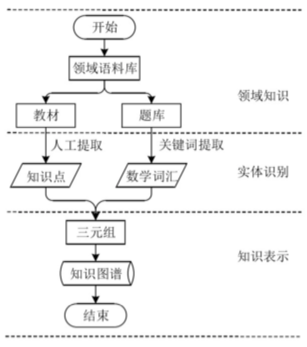
\includegraphics[width=0.8\textwidth]{./image/kg1.png}
	\caption{Structure of Triad}
	\label{kg1}
\end{figure}

\paragraph{Knowledge extraction}
Knowledge extraction is to extract valuable knowledge units from the text corpus through natural language processing and automated or semi-automated techniques. These knowledge units mainly contain entities, relationships between entities and other elements, and the required domain knowledge graph can be constructed through the relationships associated between entities.

\subparagraph{Entity Extraction}

The mathematical knowledge map built in this paper is mainly used to automatically extract knowledge points from the traditional question database when constructing the feature database, and the entity relationships involved are divided into two types: one is the concept ontology or mathematical knowledge points, and the other is the relevant mathematical vocabulary extracted from the text of the online question database.
There is no clear definition of mathematical knowledge points, which can be refined to ontology concepts or extended to each chapter of the mathematics textbook. The division of knowledge points has been the subject of a number of studies in education. Hao Guisheng believes that learners "learn objects as knowledge points", while some scholars study the definition of knowledge points from the perspective of cognitive psychology and believe that "knowledge points are human cognitive units", and discuss from the perspectives of the totality of knowledge points and human short-term memory containers The point of view that "people learn knowledge as a unit of knowledge points" is proposed, and "from the situation that people use the concept of knowledge points, a knowledge point refers to any individual piece of knowledge. According to this definition, any single word, word, concept, theorem, law, formula, law, idea, etc. can be called a knowledge point. Xie Shenquan believes that "the basic principle of dividing knowledge points is to ensure the local integrity of knowledge content, and the size of knowledge points can be arbitrary. For example, a chapter can be divided into a large knowledge point, and the content of a section can be subdivided into smaller knowledge points, and the definitions and theorems in a section can be divided into even smaller knowledge points. And the knowledge points are divided into meta-knowledge points and compound knowledge points, where meta-knowledge points refer to a formula and a definition, and compound knowledge points refer to the knowledge points formed by the combination of two or more meta-knowledge points. In this paper, we adopt Xie Shenquan's view on the definition of knowledge points and divide the knowledge points with the "General High School Mathematics Curriculum Standards". Because of the characteristics of mathematical knowledge points are relatively stable and do not change much, this paper adopts the way of manual extraction to extract the concept ontology and knowledge points of high school mathematics in order to ensure the accuracy of the knowledge points. The entity is considered as a mathematics-related term. For example, in the knowledge point of "Operations on Sets", the entities that can be associated are "union set", "intersection set", "complement set "and "cup" and "cap" in Latex format, which can be understood as mathematics-related vocabulary.
The extraction process of mathematics-related vocabulary is to first standardize the test questions in the question bank into Latex text, then perform custom dictionary priority word separation on the text by named entity recognition, filter out the deactivated words in the text by deactivated word dictionary, extract the text keywords as candidate mathematical vocabulary entities by Textr ank algorithm, and incorporate them into the knowledge graph as mathematical vocabulary entities after the expert review.

The main keyword extraction algorithms are Textr ank and TF-IDF, Textr ank is a weighting algorithm designed by Google for sentences in text, inspired by the Pagerank algorithm. TF-DF (term frequency-inverse document frequency) is mainly used in the extraction of keywords in information retrieval technology, The higher the proportion of candidate keywords appearing in the document, the larger the TF value, and the less the number of candidate keywords appearing in all texts, the larger the IDF value. The higher the proportion of candidate keywords appearing in the document, the larger the TF value, the less the number of candidate keywords appearing in all the text, the larger the IDF value, the higher the freshness, and the product of TF and IDF values of all the calculated candidate keywords in the text is sorted according to the size to obtain the importance of the candidate keywords to be extracted from the text.
TF-IDF is a purely word frequency idea (either TF or IDF) to calculate the score of a candidate keyword, and finally to extract the keyword, without considering the correlation between the candidate keywords and the semantic relationship of the keywords in the text, while Textrank algorithm takes this into account. In this paper, Textrank is used as the algorithm for extracting mathematics-related words in the mathematics question database because of the large number of semantic inferences and word associations in the text of the test questions.
Pagerank is an algorithm used by Google to calculate the importance ranking of web pages to improve the efficiency and quality of search engines. The algorithm constitutes a directed graph of web pages and links in the World Wide Web, with each web page as each node of the directed graph and links as edges of the graph.

\subparagraph{Relationship extraction}

In the study of entity extraction, the knowledge graph of high school mathematics mainly involves two entities, namely, mathematical knowledge points and related mathematical vocabulary, and the relationship between these two types of entities is associative, i.e., the knowledge points of the test questions can be found through related mathematical vocabulary. The knowledge points are divided into meta-knowledge points and compound knowledge points, so there are also knowledge points within the mathematical knowledge point entity contains the relationship 4기, for example, the mathematical knowledge point "series" contains "equal difference series" and "equal ratio series". isometric series" two knowledge points, "basic primary functions" contains "primary function", "quadratic function", "inverse function", "inverse function", "inverse function". Inverse functions", "power functions", "exponential functions", "logarithmic functions", "trigonometric functions" and so on. "Trigonometric functions" and other knowledge points.

\paragraph{The representation of knowledge}
The entities and relations required for knowledge mapping are obtained by normalizing the mathematical corpus and extracting the knowledge. In this paper, the knowledge map is represented by means of triads, which are composed of entities, attributes and relationships, among which entities and attributes can be understood as entities in the common sense, mainly consisting of meta-knowledge points, compound knowledge points and mathematics-related vocabulary, and relationships mainly consisting of the inclusion relationship between compound knowledge points and meta-knowledge points, and the association relationship between knowledge points and mathematics-related vocabulary. The RDF hierarchy of composite knowledge points, meta-knowledge points and mathematics-related vocabulary is shown in Figure \cite{2}, and function properties are shown as an example. The function properties mainly include parity, monotonicity, periodicity, symmetry, extremum, and maximum, etc. Each knowledge point corresponds to its mathematics-related vocabulary, and each knowledge point consists of its concept, corresponding chapter, corresponding artificial description, and other attributes.
\begin{figure}[h]
	\centering

	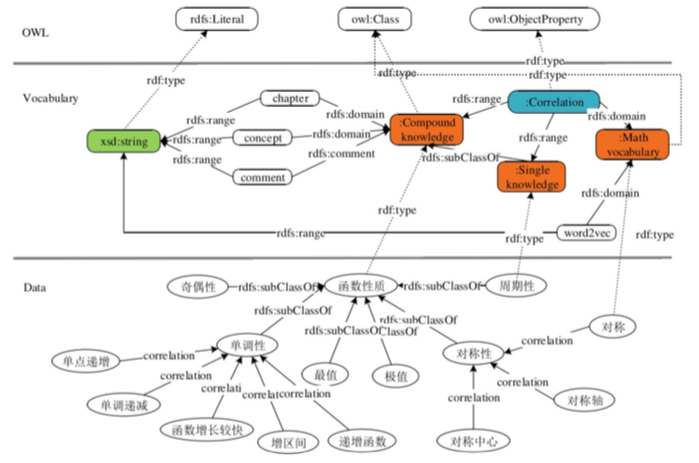
\includegraphics[width=0.8\textwidth]{./image/kg2.png}
	\caption{The representation of triad}
	\label{kg2}
\end{figure}

\paragraph{Storage}
Knowledge graph is a graph-based data structure consisting of nodes and edges, and graph databases meet such characteristics, so it has become a trend to use graph databases instead of RDF as a medium for storing knowledge graphs. Compared with RDF database, graph database is more general, in which entities are stored as nodes and relations are stored as edges.
Neoj is a new graph database developed in recent years, which belongs to NOSQL: a kind of database eo4j is an optimized graph database, with the following advantages: 

\begin{enumerate}
	\item At the same time, if the traditional relational database is used for storage, many tables are needed, and there are foreign keys and other links and constraints between the tables, which will take up a lot of physical storage space.
	\item Data presentation is more intuitive, Neoj comes with a browser and a set of easier query and operation of the Cypher language, through the Cypher language can be intuitive in the browser to view the specific relationship between the required nodes and nodes, while returning in json format, more conducive to the later operation of data.
	\item read, write and query speed, Neo4j graph database storage nodes using the Index-free Adjacency technology, that is, each node has a pointer to its neighbor nodes, allowing us to find the neighbor nodes in the case of time complexity O (1), Neo" in the edge is called First- class Entities, which are stored separately, are very convenient for graph traversal in any direction without affecting the speed of traversing the data. When an entity changes, only the content of the corresponding entity needs to be modified individually, without changing the relationship between the entity and the edge.
\end{enumerate}
In this thesis, the Neo4j graph database is used as the storage medium to store the high school mathematical knowledge map. The initial mathematical knowledge map is stored by directly importing the previously collected triad information through the Neo4j graph database client. Figure \cite{kg3} shows the global and local mathematical knowledge maps browsed by Neo4j's own browser. 

\begin{figure}[h]
	\centering

	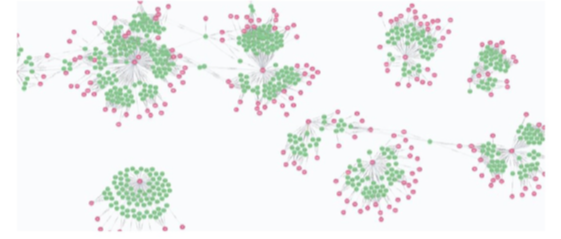
\includegraphics[width=0.8\textwidth]{./image/kg3.png}
	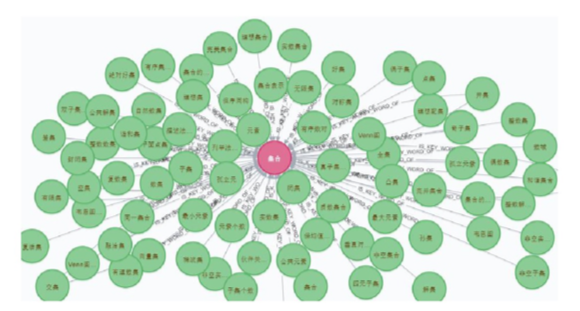
\includegraphics[width=0.8\textwidth]{./image/kg4.png}
	\caption{The knowledge graph of high school math}
	\label{kg3}
\end{figure}

\subsection{Experiment}
The accuracy of the knowledge point extraction directly affects the construction of the feature database. The experiment selected 100,000 and 500 high school mathematics test questions with knowledge points in the web crawler as samples, and divided them into two parts for the automatic extraction of knowledge points without and with expert audit. As shown in Table , the accuracy of knowledge point extraction is 72.3\% when there is no expert review and 96.6\% when there is expert review. This experiment shows that the real-time updating of the knowledge map of high school mathematics in the process of automatic knowledge point extraction is the key to improve the accuracy of knowledge point extraction.

\begin{table}[h]
	\centering

	\begin{tabular}{|l|l|l|}
	\hline
				& Without expert review & With expert review \\ \hline
	Sample Size & 100000                & 500                \\ \hline
	Accuracy    & 72.3\%                & 96.6\%             \\ \hline
	\end{tabular}
	\caption{The accuracy comparison table}
\end{table}

\subsection{Summary}
This chapter introduces the automatic knowledge extraction method of test questions based on knowledge graph. The intelligent algorithm based on individual features proposes to convert the standard question bank into a feature bank with knowledge feature representation, and defines each dimension in the feature bank, constructs the individual feature bank for users according to individual knowledge points, and explains the recommendation algorithm of test questions in the intelligent question bank; the automatic extraction method of knowledge points of test questions based on knowledge map introduces the whole process of knowledge map of high school mathematics from corpus collection, construction, storage and update. This chapter also introduces the automatic extraction process of knowledge points of high school mathematics test questions. This chapter also presents a comparative experiment on the objectivity of feature database construction and the effectiveness of automatic knowledge point extraction, and the related analysis of the experimental results.

\clearpage
\section{The GNN based knowledge tracing model}
\subsection{Background}
Knowledge tracing is a key issue in personalized learning, characterized by automation and personalization, and its task is to automatically track students' knowledge level over time based on their historical learning trajectory, so that it can accurately predict how students will perform in future learning and provide appropriate learning support. In this process, the knowledge space is used to describe the level of student knowledge acquisition. A knowledge space is a collection of concepts, and a student's mastery of a part of a collection of concepts constitutes the student's mastery of knowledge. Some educational researchers argue that students' mastery of a particular set of related knowledge points will affect their performance on the exercise, i.e., the set of knowledge that students have mastered is closely related to their external performance on the exercise. In an E-learning system, students' performance can be predicted gradually over time, and correct prediction can help students to choose the exact test questions that are comparable to their current cognitive level, and this e-learning platform can help students to improve their learning motivation. better than any of the previous methods. From a data structure perspective, course learning can also be modeled as a graph model, where the knowledge points required to master a knowledge concept proficiently are modeled as points on a graph, and these knowledge points are interrelated with each other. It is known that introducing a priori knowledge about the graph structural nature of data into the model can improve the performance and interpretability of the model.

For example, if a knowledge concept is split into three knowledge points, denoted as $V=\{v_1,v_2,v_3\}$, and to master $v_1$, it is necessary to master knowledge point $v_2$, and at the same time, to master knowledge point $v_2$, it is also necessary to master $v_3$ (for example, to solve a binary equation, it is necessary to solve a quadratic equation, and to solve a quadratic equation, it is necessary to shift terms), so the knowledge point model combined with the graph structure can effectively improve the knowledge tracing model, however, DKT does not consider this relationship between knowledge points, and previous architectures based on deep learning ground methods (e.g., RNN) usually perform well for sequential data, but cannot effectively handle graphically structured data.

Recently, research based on graph neural networks has emerged, although manipulating data on such irregular domains has challenged existing and its learning methods, and various generalization frameworks and important operations have yielded better results in several studies.GNN improves the efficiency of machine learning models from the perspective of relational induction bias, combined with human a priori knowledge of the nature of the data, a part that Battaglia et al. consider to be interpretable. GNN can find the underlying knowledge structure, but the problem is also here, how to represent the underlying knowledge structure is difficult when using graph neural networks in knowledge tracing, GNN has considerable expressive power for modeling graphically structured data. In this paper, we redefine it as a GNN application and propose a new model that can predict student knowledge mastery while considering the underlying knowledge structure.

In some cases of knowledge tracing, the relationships between knowledge points and the strength of the relationships, which are not explicitly provided, are necessary for human experts to heuristically and manually annotate the content relationships, but it takes a lot of time for a domain expert to do so. So it is difficult to model all knowledge in advance for knowledge point graphs, we define this kind of problem as hidden graph structure problem, like concept answer transfer probability, another solution is to optimize the main task while learning the graph structure itself, a related topic in recent research about GNN is the learning of graph edges (knowledge point relations).

\subsection{Concept of knowledge tracing}
% Knowledge tracing is to modeling the knowledge state of student. $y^t=KT(x^1,...,x^t),x^t=\{q^t,r^t\}$,
% $x_t$ denotes the probability $r$ of correctly answering a series of questions $q$ (vectors) at time $t$, and $y_t$ is the probability that the student correctly answers each exercise at the next time $t+1$. KT is a knowledge tracing model. This model defines a hidden state, or a state of the student's current knowledge base, and updates it continuously as the student does the questions. The model represented by RNN defines a fixed-length vector $X$, and $x_t$ is represented by two discrete values 0 and 1, where 0 means the question is wrong and 1 means the question is right, and the training goal is to minimize the negative log-likelihood (NLL) of the sequence of student responses observed under the model.

The essence of knowledge tracing is to predict students' mastery of knowledge points at any point in time based on their learning history, to predict their future performance, and to assist teachers in planning their teaching. In order to solve the knowledge tracing task, the first step is to model user interactions, and the existing modeling approaches are divided into two types based on the timing of feedback.

The first modeling approach is the user interaction modeling with real-time feedback. In some cases in reality, students need to update their knowledge in the model immediately after completing an exercise. For example, in a daily practice, students can get feedback immediately after completing an exercise and their knowledge changes. Obviously, when tracing the current moment of mastery, we should take into account all previous exercises given the student's learning history on a given task $X_t=(x_1,x_2,⋯,x_t)$ and predict the student's performance on the next exercise $x_{t+1}$, where xt is usually represented as an ordered pair $(q_t,a_t)$, the ordered pair indicates that the student answered question $qt$ at time $t$, and at indicates whether the question was answered correctly, like Figure \ref{kt1}. Each question qt will contain the textual description of the question Eq, and the knowledge point kq of the question design. DKT, EERNN, and models based on BKT extensions all use this modeling approach.

\begin{figure}[h]
	\centering
	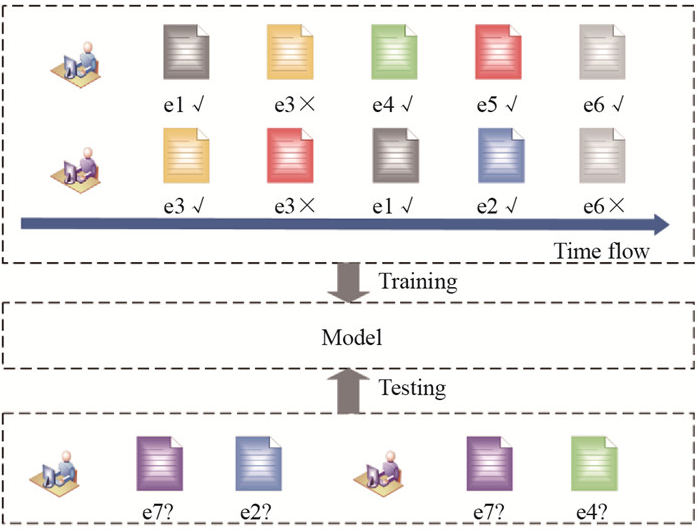
\includegraphics[width=0.8\textwidth]{./image/kt1.png}
	\caption{User interaction modeling with real-time feedback}
	\label{kt1}
\end{figure}

The second modeling approach is user interaction modeling based on stage feedback. Contrary to the previous case, in some cases students do not receive immediate feedback after completing an exercise and therefore cannot immediately update the model with information about their mastery of the knowledge. For example, in an exam, students cannot get the answer immediately after completing a question, so their mastery does not change much during the exam. In other words, in a test, the correctness of the first answer does not affect the subsequent questions, like Figure \ref{kt2} Given a student's learning history $E_t=(e_1,e_2,⋯,e_t)$, the student's performance in the next time window $e_{t+1}$ is predicted. Where $ei=(x_1,x_2,⋯,x_n)$ denotes the student's learning record in the ith time window, $n$ denotes the number of questions completed in that time period; $x_k$ denotes an ordered pair $(q_k,a_k)$, the ordered pair indicates that the student answered the kth question $q_k$ in that time window, and $a_k$ indicates whether the question was answered correctly. The length of each time window can be varied flexibly according to different needs. This modeling approach is used in KPT, PMF.

\begin{figure}[h]
	\centering
	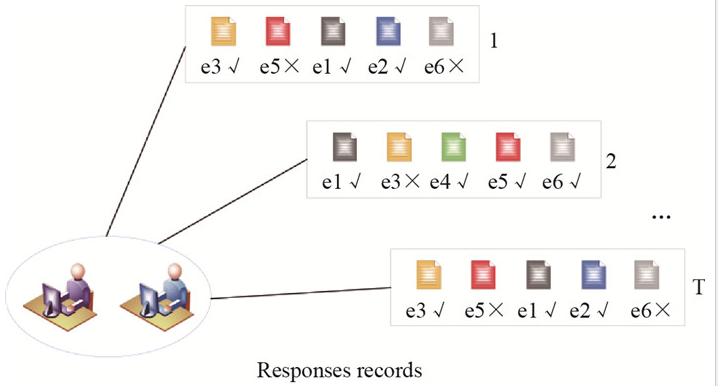
\includegraphics[width=0.8\textwidth]{./image/kt2.png}
	\caption{User interaction modeling with phased feedback}
	\label{kt2}
\end{figure}


\subsection{Survey on graph neural network}
In recent years, research on analyzing graphs by machine learning methods has received increasing attention in recent years due to the powerful expressive power of graph structures. Graph neural network (GNN) is a class of deep learning-based methods for processing graph domain information. Due to its better performance and interpretability, GNN has recently become a widely used graph analysis method.

There are five major classes of graph neural networks: Graph Convolution Networks (GCN), Graph Attention Networks(GAN), Graph Autoencoders(GAE), Graph Generative Networks(GGN), and Graph Spatial-temporal Networks(GSN).

The graph-based recommendation system uses items and users as nodes. By using item-to-item, user-to-user, and user-to-item relationships and content information, the graph-based recommendation system is able to generate high-quality recommendations. The key to a recommendation system is to evaluate the importance of an item to a user. Therefore, it can be transformed into a link prediction problem. The goal is to predict the missing links between users and items. To solve this problem, some scholars have proposed a GCN-based graphical autoencoder. Other scholars have combined GCN and RNN to learn the hidden steps of users' ratings of items.



\subsubsection{Graph Convolution Networks}
A graph convolutional network extends convolutional operations from traditional data (e.g., images) to graph data. The core idea is to learn a function mapping $f(.)$ through which a node $v_i$ in the mapping graph can aggregate its own features $x_i$ with its neighboring features $x_j$ ($j\in N(v_i)$) to generate a new representation of the node $v_i$. Graph convolutional networks are the basis for many complex graph neural network models, including autoencoder-based models, generative models, and spatio-temporal networks. The following Figure \ref{gcn1} visualizes the steps of learning node representations for graph neural networks.

\begin{figure}[h]
	\centering
	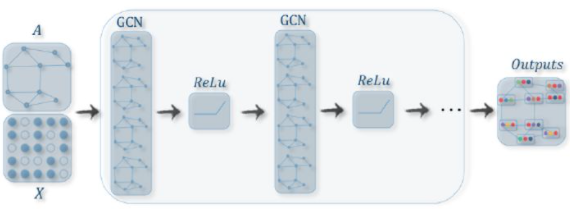
\includegraphics[width=0.8\textwidth]{./image/gcn1.png}
	\caption{A multiple GCN layers neural network}
	\label{gcn1}
\end{figure}


GCN methods can be further divided into two main categories, spectral-based and spatial-based. Spectral-based methods define graph convolution by introducing filters from the perspective of graph signal processing, where the graph convolution operation is interpreted as removing noise from the graph signal. The spatial-based approach represents graph convolution as aggregating feature information from the neighborhood. When the algorithm of the graph convolution network runs at the node level, the graph pooling module can be interleaved with the graph convolution layer to coarsen the graph into high-level substructures. As shown in the Figure \ref{gcn2}, this architectural design can be used to extract graph representations at all levels and perform graph classification tasks.


\begin{figure}[h]
	\centering
	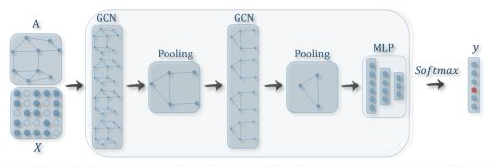
\includegraphics[width=0.8\textwidth]{./image/gcn2.png}
	\caption{GCN with pooling modules}
	\label{gcn2}
\end{figure}

\subsubsection{Graph Attention Networks}
GCN methods can be further divided into two main categories, spectral-based and spatial-based. Spectral-based methods define graph convolution by introducing filters from the perspective of graph signal processing, where the graph convolution operation is interpreted as removing noise from the graph signal. The spatial-based approach represents graph convolution as aggregating feature information from the neighborhood. When the algorithm of the graph convolution network runs at the node level, the graph pooling module can be interleaved with the graph convolution layer to coarsen the graph into high-level substructures. As shown in the figure below, this architectural design can be used to extract graph representations at all levels and perform graph classification tasks.

\paragraph{Graph Attention Network}
Graph Attention Network (GAT) is a spatially based graph convolution network that uses the attention mechanism to determine the weights of node neighborhoods when aggregating feature information.The graph convolution operation of GAT is defined as: 
$$\mathbf{h}_{i}^{t}=\sigma\left(\sum_{j \in \mathcal{N}_{i}} \alpha\left(\mathbf{h}_{i}^{t-1}, \mathbf{h}_{j}^{t-1}\right) \mathbf{W}^{t-1} \mathbf{h}_{j}^{t-1}\right)$$

where $\sigma(\cdot)$ is an attention function that adaptively controls the contribution of neighboring node j to node i. To learn the attention weights in different subspaces, GAT can also use multiple attentions.
$$\mathbf{h}_{i}^{t}=\phi_{o}\left(\mathbf{x}_{i} \oplus \|_{k=1}^{K} g_{i}^{k} \sum_{j \in \mathcal{N}_{i}} \alpha_{k}\left(\mathbf{h}_{i}^{t-1}, \mathbf{h}_{j}^{t-1}\right) \phi_{v}\left(\mathbf{h}_{j}^{t-1}\right)\right)$$

\paragraph{Gated Attention Network}
Gated Attention Network (GAAN) also employs a multi-head attention mechanism to update the hidden state of nodes. However, instead of assigning equal weights to each head part, GAAN introduces a self-attentive mechanism which calculates different weights for each head. The update rule is defined as that
$$\mathbf{h}_{i}^{t}=\phi_{o}\left(\mathbf{x}_{i} \oplus \|_{k=1}^{K} g_{i}^{k} \sum_{j \in \mathcal{N}_{i}} \alpha_{k}\left(\mathbf{h}_{i}^{t-1}, \mathbf{h}_{j}^{t-1}\right) \phi_{v}\left(\mathbf{h}_{j}^{t-1}\right)\right)$$
where $\phi_0(\cdot)$ and $\phi_v(\cdot)$ is the feedback neural network, and $g_i^k$ is the attention weight of the kth attention head

\paragraph{Graph Attention Model}
The Graph Attention Model (GAM) provides a recurrent neural network model to solve the graph classification problem by adaptively accessing a sequence of significant nodes to process information about the graph.The GAM model is defined as

$$\mathbf{h}_{t}=\mathbf{f}_{h}\left(\mathbf{f}_{s}\left(\mathbf{r}_{t-1}, \mathbf{v}_{t-1}, g ; \theta_{s}\right), \mathbf{h}_{t-1} ; \theta_{h}\right)$$

where $f_h(\cdot)$ is an LSTM network and $f_s$ is a step network that will preferentially visit neighbors with high priority of the current node $v_{t-1}$ and aggregate their information.

In addition to assigning attention weights to different neighbor nodes when aggregating feature information, it is also possible to aggregate multiple models based on attention weights, as well as to use attention weights to guide random walks. Although GAT and GAAN perform classification in the framework of graph attention networks, they can also be considered simultaneously as spatially based graph convolutional networks. the advantage of GAT and GAAN is that they are able to learn the importance weights of their neighbors adaptively. However, the computational cost and memory consumption increase rapidly with the computation of attention weights between each pair of neighbors.

\subsubsection{Graph Autoencoders}
Graph autoencoders are a class of graph embedding methods that aim to represent the vertices of a graph as low-dimensional vectors using a neural network structure. A typical solution is to use a multilayer perceptron as an encoder to obtain node embeddings, where the decoder reconstructs the neighborhood statistics of the nodes, such as positive pointwise mutual information (PPMI) or first- and second-order approximations. Recently, researchers have explored the use of GCNs as encoders, combining GCNs with GANs, or combining LSTMs with GANs to design graph autoencoders. We will first review GCN-based AutoEncoders and then summarize other variants in this category.

The main current approaches to GCN-based AutoEncoders are Graph Autoencoder (GAE) and Adversarially Regularized Graph Autoencoder (ARGA).Other variants of graph self-encoders are Network Representations with Adversarially Regularized Autoencoders (NetRA), Deep Neural Networks for Graph Representations (DNGR), Structural Deep Network Embedding (SDNE) and Deep Recursive Network Embedding (DRNE).

DNGR and SDNE learn node embeddings that give only the topology, while GAE, ARGA, NetRA, and DRNE are used to learn node embeddings when both topological information and node content features are present. One challenge of the graph autoencoder is the sparsity of the adjacency matrix A, which makes the number of positive entries of the decoder much smaller than the number of negative entries. To solve this problem, DNGR reconstructs a denser matrix, the PPMI matrix, SDNE penalizes the zero entries of the adjacency matrix, GAE reweights the entries in the adjacency matrix, and NetRA linearizes the graph into sequences.

\subsubsection{Graph Generative Networks}
The goal of graph generation networks is to generate new graphs given a set of observed graphs. Many approaches to graph generation networks are domain specific. For example, in molecular graph generation, some work simulates a string representation of molecular graphs called SMILES. In natural language processing, generating semantic graphs or knowledge graphs is usually conditional on a given sentence. Recently, several general approaches have been proposed. Some works use the generative process as an alternating factor of node and edge formation, while others use generative adversarial training. Such approaches either use GCN as a building block or use different architectures.

The main GCN-based graph generative networks are

Molecular Generative Adversarial Networks (MolGAN): integrates relational GCN, improved GAN and reinforcement learning (RL) goals to generate graphs with desired properties.The GAN consists of a generator and a discriminator that compete with each other to improve the authenticity of the generator. In MolGAN, the generator attempts to propose a pseudo-graph and its feature matrix, while the discriminator aims to distinguish between pseudo-samples and empirical data. In addition, a reward network parallel to the discriminator is introduced to encourage the generated graphs to have certain properties based on external evaluators.

Deep Generative Models of Graphs (DGMG): a space-based graph convolutional network is used to obtain a hidden representation of existing graphs. The decision process for generating nodes and edges is based on the representation of the entire graph. In short, DGMG recursively generates a node in a graph until some stopping condition is reached. At each step after adding a new node, DGMG iteratively decides whether to add an edge to the added node until the decision result of the decision becomes false. If the decision is true, the probability distribution of connecting the newly added node to all existing nodes is evaluated and a node is drawn from the probability distribution. After adding the new node and its edges to the existing graph, DGMG will update the graph representation.

The main graph generation networks of other architectures are

GraphRNN: a deep graph generation model via two levels of recurrent neural networks. The graph-level RNN adds one new node at a time to the sequence of nodes, while the edge-level RNN generates a binary sequence indicating the connection between the newly added nodes and the previously generated nodes in the sequence. To linearize a graph into a sequence of nodes to train a graph-level RNN, GraphRNN employs a breadth-first search (BFS) strategy. To build a binary sequence model for training edge-level RNNs, GraphRNN assumes that the sequence obeys a multivariate Bernoulli distribution or a conditional Bernoulli distribution.

NetGAN: Netgan combines LSTM with Wasserstein-GAN to generate graphs using a random walk based approach.The GAN framework consists of two modules, a generator and a discriminator. The generator does its best to generate reasonable random walk sequences in the LSTM network, while the discriminator tries to distinguish between the faked random walk sequences and the real random walk sequences. After training, the co-occurrence matrix of the nodes in a set of random walks is regularized and we can obtain a new graph. 

\subsubsection{Graph Spatial-Temporal Networks}
The graph spatio-temporal network simultaneously captures the spatio-temporal correlation of the spatio-temporal graph. Spatio-temporal graphs have a global graph structure where the input of each node varies with time. For example, in a traffic network, each sensor acts as a node to continuously record the traffic speed of a particular road, where the edges of the traffic network are determined by the distance between sensor pairs. The goal of graphical spatio-temporal networks can be to predict future node values or labels, or to predict spatio-temporal graph labels. Recent studies have only explored the use of GCNs, the combination of GCNs with RNNs or CNNs, and recurrent architectures tailored to graph structures.

\subsection{Proposed Model - GCKT}
In this section, we will introduce our method in detail, and the overall framework is shown in Figure \ref{GCKT1}. We first leverage GCN to learn question and skill repre- sentations aggregated on the question-skill relation graph, and a recurrent layer is used to model the sequential change of knowledge state. To capture long term dependency and exploit useful information comprehensively, we then design a recap module followed by an interaction module for the final prediction.

\begin{figure}[h]
	\centering
	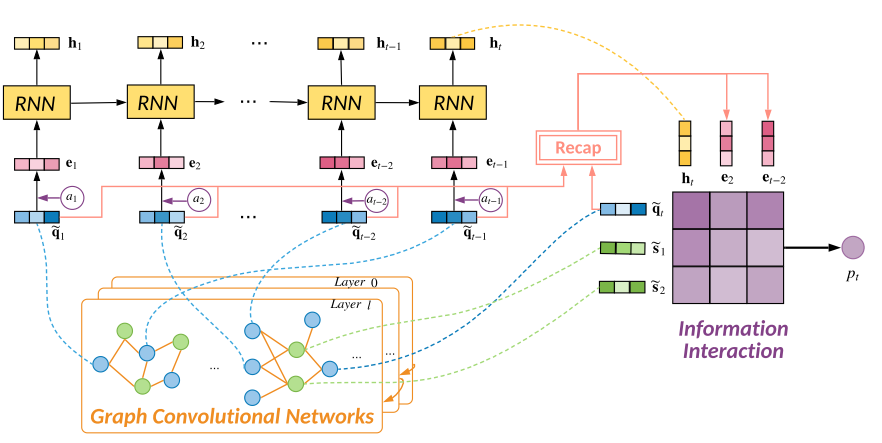
\includegraphics[width=0.8\textwidth]{./image/GCKT1.png}
	\caption{GCN-based Knowledge Tracing Model}
	\label{GCKT1}
\end{figure}

At time step t, where qt is the new question. First we use GCN to aggregate question and skill embeddings. Then a recurrent neural network is used to model the sequential knowledge state ht. In recap module we select the most related hidden exercises of qt, which corresponds to soft selection and hard selection implementation. The information interaction module performs pairwise interaction be- tween the students current state, the selected students history exercises, the target question and related skills for the prediction pt.

\subsubsection{Embedding layer}
The model uses embeddings to represent questions, skills and answers. Three embedding matrices $\mathbf{E}_{s} \in \mathbb{R}^{|\mathcal{S}| \times d}$,$\mathbf{E}_{q} \in \mathbb{R}^{|\mathcal{Q}| \times d}$,$ \mathbf{E}_{a} \in \mathbb{R}^{2 \times d}$ are denoted for look-up operation where $d$ stands for the embedding size. Each row in $E_s$ or $E_q$ corresponds to a skill or a question. The two rows in $E_a$ represent incorrect and correct answers respectively. For i-th row vector in matrices, we use $s_i$, $q_i$ and $a_i$ to represent them respectively. In our framework, we do not pretrain these embeddings and they are trained by optimizing the final objective in an end-to-end manner.

\subsubsection{Embedding Propagation}
The sparsity of the data in training can have a large impact, especially for problems where the training examples are quite limited. According to relevant pedagogical theories, whether a student answers a question correctly or not depends on the acquisition of relevant skills and knowledge points, and whether the question is close to similar questions in sequence. We address the sparsity of training by skill-question correlation graphs $\mathcal{G}$ and use the correlation of related questions to obtain better question representations.

Considering the question-skill relation graph is bipartite, the 1st hop neighbors of a question should be its corresponding skills, and the 2nd hop neighbors should be other questions sharing same skills. To extract the high-order information, we leverage graph convolutional network (GCN) to encode relevant skills and questions into question embeddings and skill embeddings.

Graph convolutional network stacks several graph convolution layers to encode high-order neighbor information, and in each layer the node representations can be updated by embeddings of itself and neighbor nodes. Denote the representation of node i in the graph as $x_i$ ($x_i$ can represent skill embedding $s_i$ or question embedding $q_i$) and the set of its neighbor nodes as $N_i$, then the formula of l-th GCN layer can be expressed as:

$$\mathbf{x}_{i}^{l}=\sigma\left(\frac{1}{\left|\mathcal{N}_{i}\right|} \sum_{j \in \mathcal{N}_{i} \cup\{i\}} \mathbf{w}^{l} \mathbf{x}_{j}^{l-1}+\mathbf{b}^{l}\right) \label{1}$$

where $w_l$ and $b_l$ are the aggregate weight and bias to be learned in l-th GCN
layer, $\sigma$ is the non-linear transformation such as ReLU. After embedding propagation by GCN, we get the aggregated embedding of questions and skills. We use $\widetilde{q}$ and $\widetilde{s}$ to represent the question and skill representation after embedding propagation. For easy implementation and better parallelization, we sample a fixed number of question neighbors (i.e., $n_q$) and skill neighbors (i.e., $n_s$) for each batch. And during inference, we run each example multiple times (sampling different neighbors) and average the model outputs to obtain stable prediction results.

\subsubsection{Individual State Evolution}
For each history time $t$, we concatenate the question and answer embeddings and project to d-dimension through a non-linear transformation as exercise representations:
$$\mathbf{e}_{t}=\operatorname{ReLU}\left(\mathbf{W}_{1}\left(\left[\widetilde{\mathbf{q}}_{t}, \mathbf{a}_{t}\right]\right)+\mathbf{b}_{1}\right) \label{2}$$
where we use $[,]$ to denote vector concatenation. There may exist dependency between different exercises, thus we need to model the whole exericise process to capture the student state changes and to learn the potential relation between exercises. To model the sequential behavior of a student doing exercise, we use LSTM to learn student states from input exercise representations:

$$
\begin{aligned}
\mathbf{i}_{t} &=\sigma\left(\mathbf{W}_{i}\left[\mathbf{e}_{t}, \mathbf{h}_{t-1}, \mathbf{c}_{t-1}\right]+\mathbf{b}_{i}\right) \\
\mathbf{f}_{t} &=\sigma\left(\mathbf{W}_{f}\left[\mathbf{e}_{t}, \mathbf{h}_{t-1}, \mathbf{c}_{t-1}\right]+\mathbf{b}_{f}\right) \\
\mathbf{o}_{t} &=\sigma\left(\mathbf{W}_{o}\left[\mathbf{e}_{t}, \mathbf{h}_{t-1}, \mathbf{c}_{t-1}\right]+\mathbf{b}_{o}\right) \\
\mathbf{c}_{t} &=\mathbf{f}_{t} \mathbf{c}_{t-1}+\mathbf{i}_{t} \tanh \left(\mathbf{W}_{c}\left[\mathbf{e}_{t}, \mathbf{h}_{t-1}\right]+\mathbf{b}_{c}\right) \\
\mathbf{h}_{t} &=\mathbf{o}_{t} \tanh \left(\mathbf{c}_{t}\right)
\end{aligned}
$$

where $h_t$, $c_t$, $i_t$, $f_t$, $o_t$ represents hidden state, cell state, input gate, forget gate, output gate respectively. It is worth mentioning that this layer is important for capturing coarse-grained dependency like potential relations between skills, so we just learn a hidden state $h_t ∈ \mathbb{R}^d$ as the current student state, which contains coarse-grained mastery state of skills.

In a student's exercise history, questions of relevant skills are very likely scattered in the long history. From another point, consecutive exercises may not follow a coherent topic. These phenomena raise challenges for LSTM sequence modeling in traditional KT methods: (i) As is well recognized, LSTM can hardly capture long-term dependencies in very long sequences, which means the current student state $h_t$ may "forget" history exercises related to the new target question $q_t$. (ii) The current student state $h_t$ considers more about recent exercises, which may contain noisy information for the new target question $q_t$. When a student is answering a new question, he/she may quickly recall similar questions he/she has done before to help him/her to understand the new question. Inspired from this behavior, we propose to select relevant history exercises(question-answer pair) $\{e_i|i \in [1, . . . , t − 1]\}$ to better represent a student’s ability on a specific question qt, called history recap module.

We develop two methods to find relevant history exercises. The first one is hard selection, i.e., we only consider the exercises sharing same skills with the new question:
$$
\mathbf{I}_{e}=\left\{\mathbf{e}_{i} \mid \mathcal{N}_{q_{i}}=\mathcal{N}_{q_{t}}, i \in [1, . ., t-1]\right\}
$$
Another method is soft selection, i.e., we learn the relevance between target question and history states through an attention network, and choose top-k states. 
$$
\mathbf{I}_{e}=\left\{\mathbf{e}_{i} \mid R_{i, t} \leq k, V_{i, t} \geq v, i \in[1, . ., t-1]\right\}
$$
where $R_{i,t}$ is the ranking of attention function $f(q_i, q_t)$ like cosine similarity, $V_{i,t}$ is the attention value and $v$ is the lower similarity bound to filter less relevant exercises.

Previous KT methods predict a student’s performace mainly according to the interaction between student state $h_t$ and question representation $q_t$, i.e., $\langle h_t, q_t\rangle$. We generalize the interaction in the following aspects: (i) we use $\langle ht, \widetilde{qt}\rangle$ to represent the student's mastery degree of question qt, ?ht,?sj? to represent the student’s mastery degree of the corresponding skill $s_{j} \in \mathcal{N}_{q_{t}}$, (ii) we generalize the interaction on current student state to history exercises, which reflect the relevant history mastery i.e., $\left\langle\mathbf{e}_{i}, \widetilde{\mathbf{q}}_{t}\right\rangle$ and $\langle e_i,\widetilde{s_j}\rangle$, $e_i \in\mathcal{I}_e$, which is equivalent to let the student to answer the target question in history timesteps. 

Then we consider all above interactions for prediction, and define the generalized interaction module. In order to encourage relevant interactions and reduce noise, we use an attention network to learn bi-attention weights for all interaction terms,
$$\begin{aligned} \alpha_{i, j} &=\operatorname{Softmax}_{i, j}\left(\boldsymbol{W}^{T}\left[\boldsymbol{f}_{i}, \boldsymbol{f}_{j}\right]+b\right) \\ p_{t} &=\sum_{\boldsymbol{f}_{i} \in \mathbf{I}_{e} \cup\left\{\mathbf{h}_{t}\right\}} \sum_{\boldsymbol{f}_{j} \in \widetilde{\mathbf{N}}_{q_{t}} \cup\left\{\widetilde{\mathbf{q}}_{t}\right\}} \alpha_{i, j} g\left(\boldsymbol{f}_{i}, \boldsymbol{f}_{j}\right) \end{aligned}$$

where $p_t$ is the predicted probability of answering the new question correctly, $\widetilde{\mathbf{N}}_{q_{t}}$ represents the aggregated neighbor skill embeddings of qt and we use innerproduct to implement function g. Similar to the selection of neighbors in relation graph, we set a fixed number of $\mathbf{I}_{e}$ and $\widetilde{\mathbf{N}}_{q_{t}}$by sampling from these two sets.

To optimize our model, we update the parameters in our model using gradient descent by minimizing the cross entropy loss between the predicted probability of answering correctly and the true label of the student’s answer:
$$\mathcal{L}=-\sum_{t}\left(a_{t} \log p_{t}+\left(1-a_{t}\right) \log \left(1-p_{t}\right)\right)$$

\subsection{Experiment}
In this section, we conduct several experiments to investigate the performance of our model. We first evaluate the prediction error by comparing our model with other baselines on three public datasets. Then we make ablation studies on the GCN and the interaction module of GIKT to show their effectiveness. Finally, we evaluate the design decisions of the recap module to investigate which design performs better.

\subsubsection{Dataset}
To evaluate our model, the experiments are conducted on three widely-used datasets in KT and the detailed statistics are shown in Table \ref{datasetstb1}.
\begin{table}[h]
	\centering
	\caption{Dataset statistics}
	\label{datasetstb1}
	\begin{tabular}{cccc}
	
		\hline & ASSIST09 & ASSIST12 & EdNet \\
		\hline students & 3,852 & 27,485 & 5000 \\
		questions & 17,737 & 53,065 & 12,161 \\
		skills & 123 & 265 & 189 \\
		exercises & 282,619 & 2,709,436 & 676,974 \\
		questions per skill & 173 & 200 & 147 \\
		skills per question & 1.197 & 1.000 & 2.280 \\
		attempts per question & 16 & 51 & 56 \\
		attempts per skill & 2,743 & 10,224 & 8,420 \\
		\hline
	\end{tabular}
\end{table}
\begin{itemize}
	\item ASSIST094 was collected during the school year 2009-2010 from ASSISTments online education platform5. We conduct our experiments on "skill- builder" dataset. Following the previous work, we remove the duplicated records and scaffolding problems from the original dataset. This dataset has 3852 students with 123 skills, 17,737 questions and 282,619 exercises.
	\item ASSIST126 was collected from the same platform as ASSIST09 during the school year 2012-2013. In this dataset, each question is only related to one skill, but one skill still corresponds to several questions. After the same data processing as ASSIST09, it has 2,709,436 exercises with 27,485 students, 265 skills and 53,065 questions.
	\item EdNet7 was collected by Choi. As the whole dataset is too large, we randomly select 5000 students with 189 skills, 12,161 questions and 676,974 exercise
\end{itemize}

\subsubsection{Baselines}
In order to evaluate the effeciveness of our proposed model, we use the following models as our baselines. 
\begin{itemize}
	\item BKT uses Bayesian inference for prediction, which models the knowledge state of the skill as a binary variable.
	\item KTM is the latest factor analysis model that uses Factorization Machine to interact each feature for prediction. Although KTM can use many types of feature, for fairness we only use question ID, skill ID and answer as its side information in comparison.
	\item DKT is the first method that uses deep learning to model knowldge tracing task. It uses recurrent neural network to model knowldge state of students.
	\item DKVMN uses memory network to store knowledge state of different concepts respectively instead of using a single hidden state.
	\item DKT-Q is a variant of DKT that we change the input of DKT from skills to questions so that the DKT model directly uses question information for prediction.
    \item DKT-QS is a variant of DKT that we change the input of DKT to the concatenation of questions and skills so that the DKT model uses question and skill information simultaneously for prediction.
	\item GAKT is a variant of the model Exercise-Enhanced Recurrent Neural Net- work with Attention mechanism (EERNNA) as EERNNA utilizes ques- tion text descriptions but we can't acquire this information from public datasets. Thus we utilize our input question embeddings aggregated by GCN as input of EERNNA and follow its framework design for comparison.
\end{itemize}

\subsubsection{Performance}
Table \ref{auctb1} reports the AUC results of all the compared methods. From the re- sults we observe that our GIKT model achieves the highest performance over three datasets, which verifies the effectiveness of our model. To be specific, our proposed model GIKT achieves at least 1\% higher results than other baselines. Among the baseline models, traditional machine learning models like BKT and KTM perform worse than deep learning models, which shows the effectiveness of deep learning methods. DKVMN performs slightly worse than DKT on average as building states for each concept may lose the relation information between concepts. Besides, GAKT performs worse than our model, which indicates that exploiting high-order skill-question relations through selecting the most related exercises and performing interaction makes a difference. On the other hand, we find that directly using questions as input may achieve

superior performance than using skills. For the question-level model DKT-Q, it has comparable or better performance than DKT over ASSIST12 and EdNet datasets. However, DKT-Q performs worse than DKT in ASSIST09 dataset. 
\begin{table}[h]
	\centering
	\caption{AUC results over three datasets}
	\label{auctb1}
	\begin{tabular}{cccc}
		\hline Model & ASSIST09 & ASSIST12 & EdNet \\
		\hline BKT & 0.6571 & 0.6204 & 0.6027 \\
		KTM & 0.7169 & 0.6788 & 0.6888 \\
		DKVMN & 0.7550 & 0.7283 & 0.6967 \\
		DKT & 0.7561 & 0.7286 & 0.6822 \\
		\hline DKT-Q & 0.7328 & 0.7621 & 0.7285 \\
		DKT-QS & 0.7715 & 0.7582 & 0.7428 \\
		GAKT & 0.7684 & 0.7652 & 0.7281 \\
		\hline GIKT & $\mathbf{0 . 7 8 9 6}^{*}$ & $\mathbf{0 . 7 7 5 4}^{*}$ & $\mathbf{0 . 7 5 2 3}^{*}$ \\
		\hline	
	\end{tabular}
\end{table}

Among these models, BKT, DKT and DKVMN predict for skills, other models predict for questions. Note that "*" indicates that the statistically significant improvements over the best baseline, with p-value smaller than 10−5 in two-sided t-test. Reason may be that the average number of attempts per question in ASSIST09 dataset is significantly less than other two datasets as observed in Table 1, which illustrates DKT-Q suffers from data sparsity problem. Besides, the AUC results of the model DKT-QS are higher than DKT-Q and DKT, except on ASSIST12 as it is a single-skill dataset, which indicates that considering question and skill information together improves overall performance.

\subsection{Summary}
In this chapter, we propose a knowledge tracing model to employ high-order question-skill relation graphs into question and skill representations. Besides, to model the student's mastery for the question and related skills, we design a recap module to select relevant history states to represent student's ability. Then we extend a generalized interaction module to represent the student's mastery degree of the new question and related skills in a consistent way. 


\clearpage
\section{Learning Resource Recommendation System Based on Deep Factorization Machine}
This section proposes a model DeepFM model consisting of a deep neural network and a factorization machine (to implement a recommendation system for learning resources. The factorizer part mainly extracts first-order and second-order features, and the deep neural network part mainly extracts higher-order features

\subsection{Theory}
\subsubsection{Prediction task}
 In machine learning, prediction is one of the most fundamental tasks, by which is meant estimating a function.


$$
f: R^{n} \rightarrow T
$$
This function maps a dimensional vector of real-valued features $x\in R^n$ to a target domain $T$, e.g., for regression $T=R$, for classification problems$T=+,-$. In a supervised learning scenario, there is usually a labeled training data set.
$$D=\left\{\left(x^{(1)}, y^{(1)}\right),\left(x^{(1)}, y^{(1)}\right), \ldots,\left(x^{(m)}, y^{(m)}\right)\right\}$$

where $x^{(i)}\in R^n$ denotes the input data, corresponding to the feature vector of the sample, $y^{(i)}$ corresponding to the label, and $m$ is the number of samples. In the real world, many application problems generate highly sparse data, i.e., almost all components of the feature vector $x^{(i)}$ are zero.

\subsection{Factorization Machine Model}
Factorization Machine (FM) was first proposed in 2010 by Konstanz University SteffenRendle (now at Google) in 2010, which was first proposedIt aims to solve the problem of feature combination with sparse data. The FM model is comparable toThe FM model is equivalent to introducing a second-order combination term $x_i,x_j$ based on the LR model, and the formulais as follows.

$$
y(x)=\omega_{0}+\sum_{i=1}^{n} \omega_{i} x_{i}+\sum_{i=1}^{n} \sum_{j=i+1}^{n} \omega_{i j} x_{i} x_{j}
$$

where $n$ represents the number of features in the sample, $x_i$ is the value of the i-th feature, and
$ω_0, ω_i, ω_{ij}$ are the model parameters.

The polynomial model is the most intuitive model that contains a combination of features. In the polynomial model, the combination of features $x_i$ and $x_j$ is represented by $x_i x_j$, i.e., the combination of features xixj is meaningful when both xi and xj are non-zero. We can see that there are $\frac{n(n-1)}{2}$ parameters of the combined features, and any two parameters are independent. However, in practical application scenarios where data sparsity prevails, the training of the quadratic parameters is very difficult. The reason is that the training of each parameter $ω_{ij}$ requires a large number of samples with non-zero $x_i$ and $x_j$; and the sample data is already sparse, so there will be very few samples that satisfy "$x_i$ and $x_j$ are non-zero". The lack of training samples will easily lead to the inaccuracy of the parameter $ω_{ij}$, which will seriously affect the performance of the model. Therefore, a hidden vector is introduced here, and the hidden vector of the i-th dimensional feature is $v_i$, $v_i$ is a K-dimensional vector, and  $ω_{ij}$ is replaced by $\langle v_i, v_j\rangle$ to obtain the formula of the new FM model as follows.
$$
y(x)=\omega_{0}+\sum_{i=1}^{n} \omega_{i} x_{i}+\sum_{i=1}^{n} \sum_{j=i+1}^{n}\left\langle v_{i}, v_{j}\right\rangle x_{i} x_{j}
$$
The number of parameters of the binomial can be known from $\frac{n(n-1)}{2}$ decreasesto $kn$. The original binomial parameters are independent of each other, such as ωmiand ωij , using the hidden vector dot product form as $〈vm, vi〉$ and $〈vi, vj〉$, whichcontains the common term $v_i$, i.e., the parameters of $x_m x_i$ and $x_i x_j$ are no longer independent of each other. All binomial features combined with $x_i$ can be used to learn the hidden vector $v_i$.In the computation, the following equation can be used for optimization, which can reduce the timeThe time complexity can be reduced from$ O(kn2)$ to $O(kn)$.
$$
\sum_{i=1}^{n} \sum_{j=i+1}^{n}\left\langle v_{i}, v_{j}\right\rangle x_{i} x_{j}=\frac{1}{2} \sum_{f=1}^{k}\left(\left(\sum_{i=1}^{n} v_{i, f} x_{i}\right)^{2}-\sum_{i=1}^{n} v_{i, f}^{2} x_{i}^{2}\right)
$$

\subsection{DeepFM Model}
The FM model is improved on the basis of the logistic regression model and proposes to express the combinatorial features by using the hidden vector as the inner product, but in practical applications. In practical applications, however, only second-order combinatorial features are generally extracted due to the computational complexity. The focus of the advertising. The focus of the advertising lick-through rate problem is on how to mine the combination, which includes second-order, third-order and even higher-order features, and the higher the order, the more complex and less.T e higher the order, the more complex and difficult it is to learn, and the performance of learning these two combined features at the same time is better than only
The performance of learning these two combined features at the same time is better than considering only one of them. Therefore, in this paper, we propose a method consisting of a deep
Therefore, this paper proposes a model consisting of a deep neural network and a factorization machine --- DeepFM model.
Figure 1 shows the architecture of DeepFM model.

\begin{figure}[h]
	\centering
	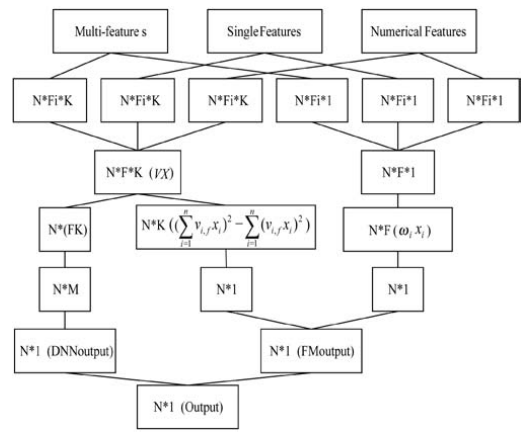
\includegraphics[width=0.8\textwidth]{./image/deepfm.png}
	\caption{The structure of DeepFM model}
	\label{deepfm}
\end{figure}

From Fig. \ref{deepfm}, we can see that the DeepFM model is mainly divided into two parts: The DeepFM model is divided into 2 parts: FM part and deep neural network part, where FM contains primary and secondary terms. The FM contains primary and secondary terms. The embedding layer is introduced in the deep neural network to compress the input vector into a low-dimensional dense vector, i.e., the hidden vector proposed in FM, which solves the problem of data sparsity on the one hand, and avoids the problem of excessive dimensionality after one-hot coding of multi-category features on the one hand, and on the other hand, avoids the problem of excessive dimensionality after one-hot encoding of multi-category features.
The quadratic terms of the DNN part and FM part share the same input, and the final training is performed simultaneously, with the following results.
$$\widetilde{y}  = Sigmoid (y_{FM} + y_{DNN}) $$
where: $y_{FM}$ represents the output of the FM part, $y_{DNN}$ represents the output of the deep neural network part. The result is transformed into a number between 0 and 1 by a Sigmoid function. 1 to obtain the final click rate prediction. 

\subsection{Experiment}
The dataset used in this paper is mainly from the public dataset, which has about 8 million users and contains 1 numerical feature and 31 class-type features (including 11 multi-value class-type features). Because of the imbalance between positive and negative samples (the ratio of positive and negative samples is about 1:20), the model is evaluated by using AUC score, which is defined as the area enclosed by the coordinate axis under the ROC curve, and the horizontal and vertical coordinates of the ROC curve are false positive rate (FPR: $\frac{FP}{TN+FP}$) and true positive rate (TPR: $\frac{TP}{TP+FN}$). 
The AUC score can be interpreted as the probability that a positive sample is ranked ahead of a negative sample, and the AUC value is 1 when the prediction result is exactly correct, so a larger AUC value indicates a more accurate classification result. Table 1 shows the confusion matrix.


\begin{table}[h]
	\centering
	\caption{Comfusion Matrix}
	\begin{tabular}{|c|c|c|}
		\hline \multirow{2}{*} {\text { Predict-Actual }} & \multicolumn{2}{|c|} {\text { Predict }} \\
		\cline { 2 - 3 } & \text { Positive } & \text { Negative } \\
		\hline \text { True } & \text { TP } & \text { FP } \\
		\hline \text { False } & \text { FN } & \text { TN } \\
		\hline
		\end{tabular}	
\end{table}

In this experiment, three models were trained for several times, and the final results were taken as the average AUC values of multiple experiments. The outcome is like Table \ref{roc1tb} and Figure \ref{roc1fg}
\begin{table}[h]
	\centering
	\caption{The original dataset outcome}
	\label{roc1tb}
	\begin{tabular}{|c|c|}
		\hline Model & AUC Value \\
		\hline LR & 0.724135 \\
		\hline FM & 0.736323 \\
		\hline DeepFM & 0.749123 \\
		\hline
	\end{tabular}
\end{table}

\begin{figure}[h]
	\centering
	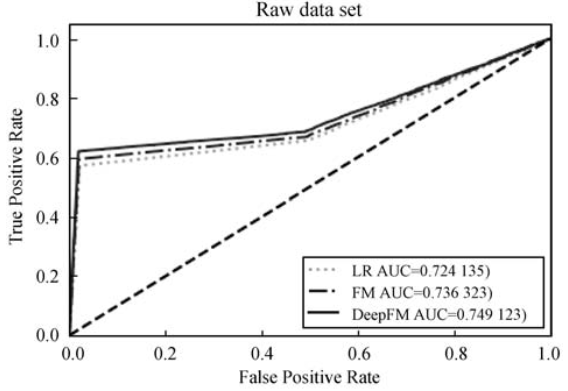
\includegraphics[width=0.8\textwidth]{./image/roc1.png}
	\caption{The ROC curve of original dataset}
	\label{roc1fg}
\end{figure}

From the results in Table \ref{roc1tb}, we can see that the FM model has higher AUC values than the LR model due to the introduction of second-order The Dep FM model has a higher AUC value than the LR model because of the introduction of second-order features, while the Dep FM model has a higher AUC value than both the LR and FM models because of the inclusion of a deep neural network to partially learn higher-order feature combinations. Analyzing Figure \ref{roc1fg}, we can see that the front of the ROC curve is approximately the straight line x=0 because of the imbalance of positive and negative samples, and the true rate of DepFM is higher than that of LR and FM at the back of the ROC curve, so the AUC value of DepFM is higher than that of both LR and FM. The results in Table \ref{roc1tb} and Fig. \ref{roc1fg} show that the DepFM model can effectively mine the higher-order combinatorial features, which is better than the LR model and FM model in terms of recommendation.

In practice, the logistic regression model as a linear model is more dependent on the manually extracted combinatorial features, so in this paper, based on the original features, an improved xk method is used to extract new combinatorial features with GBDT to supplement the data set, and the final results are shown in Table \ref{roc2tb} and Figure \ref{roc2fg}.

\begin{table}
	\centering
	\caption{Compensation dataset outcome}
	\label{roc2tb}
	\begin{tabular}{|c|c|}
		\hline Model & AUC Value \\
		\hline GBDT + LR & 0.741241 \\
		\hline GBDT + FM & 0.751732 \\
		\hline GBDT + DeepFM & 0.757137 \\
		\hline
	\end{tabular}
\end{table}

\begin{figure}[h]
	\centering
	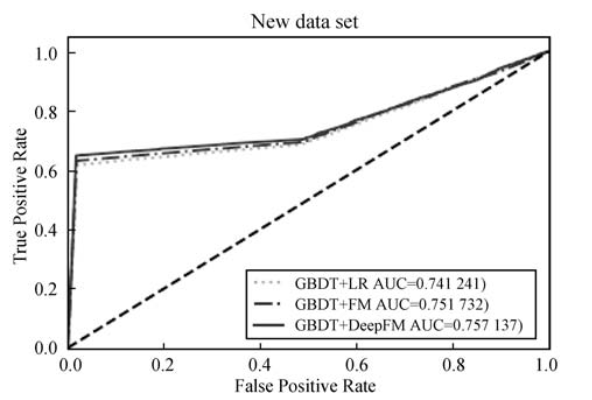
\includegraphics[width=0.8\textwidth]{./image/roc2fg.png}
	\caption{The ROC curve of new dataset}
	\label{roc2fg}
\end{figure}

From Table \ref{roc2tb} and Figure \ref{roc2fg}, we can see that the performance of the three models improves with the addition of the combination features. This is because the LR model does not introduce combinatorial features, so the performance of the LR model has improved significantly with the addition of combinatorial features; the FM and De epFM models can automatically combine features through the model structure, but the explicit addition of these features can reduce the difficulty of training the model.


\subsection{System Design}
TODO...

\subsection{Summary}
TODO...

\clearpage
\section{Conclusion}
In this paper, we propose a recommendation system design based on knowledge tracking and factorization machine to address the needs of learning resource recommendation system and the shortcomings of current online recommendation system such as single structured and lack of mining. Its core business consists of three major functional modules: learning resource knowledge map, knowledge tracking module and recommendation module. The learning resource knowledge map abstracts the existing learning resources into a graphical knowledge map by means of entity identification and relationship extraction. In the knowledge tracking module, a new knowledge tracking model based on graph neural network is proposed, and good performance and effect are achieved. In the recommendation module part, the deep factorization machine algorithm is used to solve the problem of sparsity of training data.

The main work of this paper includes:
...



\clearpage
\bibliography{wpref}

\appendix
%\appendixpage
\addappheadtotoc



\end{document}
